%%%%%%%%%%%%%%%%%%%%%%%%%%%%%%%%%%%%%%%%%%%%%%%%%%%%%%%%%%%%%%%%%%%%%%%%%%%%%%%
% Use the ``draft'' option to compile more quickly. Remove the ``twoside''
% argument if you want fewer blank pages (e.g. for an online-only version).
\documentclass{vera-ornltm}
%\documentclass[draft,twoside]{ornltm}

%\reportdraft

% Uncomment these to hide a particular page.
%\renewcommand\makeostipage\relax
%\renewcommand\makecoverpage\relax
%\renewcommand\maketitlepage\relax

% Optional packages that are simply part of this example document
\usepackage{threeparttable} % Table with captions and tablenotes
\usepackage{booktabs} % Toprule, midrule, bottomrule
\usepackage{multirow} % Extend table entries over multiple rows

% Bibliography styling. WARNING: the biblatex-chicago package removes the
% footnote rule.
% \usepackage[authordate,strict,backend=biber,autolang=other,bibencoding=inputenc]{biblatex-chicago}

% Use inline small italic blue for comments rather than placing them in the
% margin.
\definecolor{note}{RGB}{48,96,192}
\renewcommand{\marginpar}[1]{{\small\em\color{note}[#1]}}

\usepackage{amssymb}
\usepackage[mathcal]{euscript}
\usepackage{array}
\usepackage{multirow}
\usepackage{cite}
\usepackage{subcaption}
\usepackage{longtable}
\usepackage{placeins}
\usepackage{enumitem}
\usepackage{authblk}

% Define commands used in this document
% Define whatever local commands you want here

\newcommand{\invcm}{\ensuremath{\text{cm}^{-1}}}
\newcommand{\bsig}{\ensuremath{\bar{\sigma}}}
\newcommand{\bphi}{\ensuremath{\bar{\phi}}}
\newcommand{\diff}{\ensuremath{\mathrm{d}}}
\newcommand{\shift}{\texttt{Shift}}
\newcommand{\triton}{\texttt{Triton}}
\newcommand{\griffin}{\texttt{Griffin}}
\newcommand{\scale}{\texttt{SCALE}}
\newcommand{\serpent}{\texttt{Serpent}}
\newcommand{\mpact}{\texttt{MPACT}}
\newcommand{\vera}{\texttt{VERA}}



% Ensure that the list of figures (lof) and list of tables (lot) are evenly spaced
% regardless of if they are located in different sections. If that behavior is not desired,
% comment out the corresponding lof or lot line.
\newcommand*{\noaddvspace}{\renewcommand*{\addvspace}[1]{}}
\addtocontents{lof}{\protect\noaddvspace}
\addtocontents{lot}{\protect\noaddvspace}

%%%%%%%%%%%%%%%%%%%%%%%%%%%%%%%%%%%%%%%%%%%%%%%%%%%%%%%%%%%%%%%%%%%%%%%%%%%%%%%
% AUTHORSHIP & PUBLISHING
%%%%%%%%%%%%%%%%%%%%%%%%%%%%%%%%%%%%%%%%%%%%%%%%%%%%%%%%%%%%%%%%%%%%%%%%%%%%%%%

% Specify authors below.
\author{Aaron Graham}
\affil{Oak Ridge National Laboratory}

% Specify title.
% Note: if using an explicit linebreak in the title, you must use the \protect
% command before it.
\title{VERAIn Programmer's Manual 4.4}

% Specify date of publication.
\date{May 31, 2022}
%\date{\today}

% Define report number.
% Note: Defining the report number causes the 'draft' notices to be removed.
% Remove comment "%" below if that is desired.
 \reportnum{ORNL/SPR-2023/3093}

% Add a restriction notice to the cover page. Remove comment "%" below if that
% is desired.
%\restrict{Official use only}
%\restrict{Business Sensitive}
% \restrict{Not for public release.}

%%%%%%%%%%%%%%%%%%%%%%%%%%%%%%%%%%%%%%%%%%%%%%%%%%%%%%%%%%%%%%%%%%%%%%%%%%%%%%%
% ABBREVIATIONS
%%%%%%%%%%%%%%%%%%%%%%%%%%%%%%%%%%%%%%%%%%%%%%%%%%%%%%%%%%%%%%%%%%%%%%%%%%%%%%%
% Note that Abbreviations that aren't used in the document won't be printed in the
%  list.
\makeglossaries
\newacronym{3d}{3D}{three dimensional}
\newacronym{doe}{DOE}{US Department of Energy}
\newacronym{nrc}{NRC}{US Nuclear Regulatory Commission}
\newacronym{tm}{TM}{technical memo}
\newacronym{ornl}{ORNL}{Oak Ridge National Laboratory}
\newacronym{lwr}{LWR}{light-water reactor}

%%%%%%%%%%%%%%%%%%%%%%%%%%%%%%%%%%%%%%%%%%%%%%%%%%%%%%%%%%%%%%%%%%%%%%%%%%%%%%%
% FRONT MATTER
%%%%%%%%%%%%%%%%%%%%%%%%%%%%%%%%%%%%%%%%%%%%%%%%%%%%%%%%%%%%%%%%%%%%%%%%%%%%%%%
\begin{document}
\frontmatter

%Add the revision log and page descriptions
\revisionlog{
0 & 5/31/2022 & All & New template and editorial updates for VERA 4.3 release.
This version supersedes previous document version CASL-U-2019-1884-001. \\
}{None}{None}{None}{All}

%Here's how to add a signature page (class provides 2, 3, 4, or 5 signatures)
\signaturepagetwo{Aaron Graham, VERAIO Product Software Manager}{Bob Salko, Independent Reviewer}

\addcontentsline{toc}{section}{Executive Summary}
\section*{Executive Summary}

This document provides information needed by developers who will be working in the VERAIn source code. 
It provides a high-level overview of input design, as well as guidelines for adding new inputs.

\tableofcontents
% LIST OF FIGURES: optional if fewer than 5 are used
%\listoffigures
% \marginpar{The list of figures tables may be omitted if fewer than 5 are used.}
% LIST OF TABLES: optional if fewer than 5 are used
%\listoftables
% \marginpar{The list of tables may be omitted if fewer than 5 are used.}
% LIST OF ABBREVIATIONS
% NOTE: this will only print if `makeindex X.ist -o X.acr X.acn` is executed.
% This is part of the included Makefile.
%\printacronyms[title=Abbreviations]

%%%%%%%%%%%%%%%%%%%%%%%%%%%%%%%%%%%%%%%%%%%%%%%%%%%%%%%%%%%%%%%%%%%%%%%%%%%%%%%
% DOCUMENT CONTENT
%%%%%%%%%%%%%%%%%%%%%%%%%%%%%%%%%%%%%%%%%%%%%%%%%%%%%%%%%%%%%%%%%%%%%%%%%%%%%%%
\mainmatter
\section{VERAIn}

The VERAIn repository is used to translate the user-defined ASCII input file to a ParameterList XML file to be read by codes within VERA. 
The ParameterList format is defined in Trilinos Teuchos package at\\
https://docs.trilinos.org/dev/packages/teuchos/doc/html/index.html\#TeuchosParameterList\_src.
The VERAIn parser is a PERL script that translates the individual variables specified in YAML files. 
These YAML files are located in the \texttt{VERAIO/verain/scripts/Templates} directory.
To perform the translation, use the parser located in the scripts directory. 
Run the parser with a command line like the following:

\texttt{VERAIO/verain/scripts/react2xml.pl \$CASE.inp \$CASE.xml}

where \texttt{\$CASE} is the base name of the input file. 
Parser error messages indicate errors in the input file. 
Various input parameter examples can be found in the \texttt{VERAIO/verain/test} directory.

The react2xml command line options can be viewed by using

\begin{verbatim}
    react2xml.pl --help
\end{verbatim}

resulting in:

\begin{verbatim}
Converts reactor input file (reactor_input_file) into ParameterList
XML file (output_xml_file). ParameterList format is defined in
Trilinos Teuchos package: https://docs.trilinos.org/dev/packages/teuchos/doc/html/
index.html#TeuchosParameterList_src

Program error messages indicate errors in the input file.

Program switches:

--help    This help.

--xml=(on|off)
          Write XML declaration as the first line of the ParameterList
          XML file. Default=on.

--xslt=(on|off)
          Write XSLT processing instruction as the second line of the
          ParameterList XML file. Turns on --xml switch, as well. XSLT
          style file PL9.xsl should be in the same directory as the
          resulting ParameterListXML file in order for transformation
          to work in a browser. Default=on.

--verbose Add processing printouts as the code executes.

--debug   Create debug files for finding the errors in the converter
          program. Does not help much in tracing invalid input.

--schema Write the VERAIn input schematic to STDOUT formatted as JSON.
\end{verbatim}

%%%%%%%%%%%%%%%%%%%%%%%%%%%%%%%%%%%%%%%%%%%%%%%%%%%%%%%%%%%%%%%%%%%%%%%%%%%%%%%

\section{VERAIn Output}

Upon completion, several output files may be created, depending on the code options used.
Some typical outputs include the following:
\begin{itemize}
\item \textbf{VERAIn XML file:}  file written upon the successful completion of VERAIn
\item \textbf{VERA HDF output file:}  a binary file with results that can be visualized in VERAView or post-processed with user utility codes
\item \textbf{MPACT output file:} file written upon the successful completion of MPACT (if applicable)
\item \textbf{MPACT log file:} file written upon the successful completion of MPACT (if applicable)
\item \textbf{MPACT summary file:} file written upon the successful completion of MPACT (if applicable).
\item \textbf{standard output file:} a log of all output written to the standard output
\item \textbf{standard error file:} a log of all output written to the standard error file
\end{itemize}


In case of errors, the user should examine the standard error file first.
If there are any errors in the input processor (VERAIn), then they will be written here.
Any error messages from other VERA components will also be written to the standard error file.

If the standard error file does not list any errors, then check the VERA component output files and log files for messages.

%%%%%%%%%%%%%%%%%%%%%%%%%%%%%%%%%%%%%%%%%%%%%%%%%%%%%%%%%%%%%%%%%%%%%%%%%%%%%%%

\section{Style Guide}

\subsection{Adding New Variables}

This section provides instructions for adding or modifying inputs to be used in the user-provided ASCII input. For most cases, to add a new variable to the input, only the template files found in\\
\texttt{VERAIO/verain/scripts/Templates} must be modified. Generally, two files must be modified for every new input variable:
\begin{itemize}
    \item{Directory.yml}---describes how to read the inputs
    \item{BLOCK.yml}---describes how to convert inputs to parameter names for a particular BLOCK
\end{itemize}

The different BLOCK options available in an input file are:

\texttt{STATE}, \texttt{BRANCH}, \texttt{TRANSIENT}, \texttt{CORE}, \texttt{ASSEMBLY}, \texttt{CONTROL}, \texttt{INSERT}, \texttt{DETECTOR}, \texttt{EDITS}, \texttt{SHIFT}, \texttt{COBRATF}, \texttt{COUPLING}, \texttt{MPACT}, \texttt{BISON}, \texttt{FAST}, \texttt{MAMBA}, and \texttt{RUN}

For example, if a new variable is to be added to the ASSEMBLY block of the user input, then it must be added to the ASSEMBLY section of the Directory.yml file, as well as to the ASSEMBLY.yml file. 

If a new variable is added to the Directory.yml file, proper documentation must also be provided. The input description must precede the variable and must be in the following form using \LaTeX\ formatting:

\begin{small}
\begin{verbatim}
#>
#>   {\bf variable\_name} detailed\_input\_name
#>   \VERAInputTable{
#>     name={detailed\_input\_name},
#>     type={variable type: Float, Boolean, Integer... etc.},
#>     need={Optional or Required},
#>     unitsdefault={Default units for this variable},
#>     unitsother={Other acceptable units for this variable},
#>     valuedefault={Default value for this variable, if there is one},
#>     valuesapplicable={Defines acceptable values, or range of values, that this variable 
#>        can be defined as},
#>     limitations={A description of the limitations of this variable, if applicable},
#>     description={A detailed description of this variable and what it is used for.},
#>     notes={Any additional information about this variable that was not specified earlier}
#>   }
\end{verbatim}
\end{small}

It is strongly advised that a new variable include a \texttt{\_check:} section that checks to ensure that a given variable is the proper type and within the expected input variable range. An example of a two-variable input with description is shown in Figure \ref{fig:Directory_example}. This example input, \texttt{b10}, is located in the STATE block. Therefore, the corresponding entries in the STATES.yml file are shown in Figure \ref{fig:States_example}. The names given in the BLOCK.yml file will correspond to the variable name that will be given in the ParameterList XML file. 

\begin{figure}
   \centering
   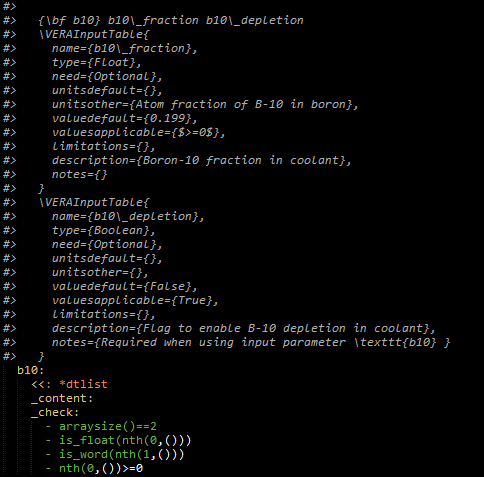
\includegraphics[width=\textwidth]{images/Directory_example}
   \caption{\label{fig:Directory_example}Example b10 inputs and descriptions in Directory.yml}
\end{figure}

\begin{figure}
   \centering
   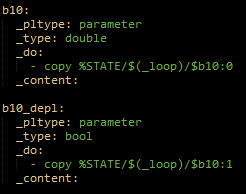
\includegraphics[width=10cm]{images/States_example}
   \caption{\label{fig:States_example}Example b10 inputs in STATES.yml }
\end{figure}
   
\subsection{Testing New Variables}

If a new input is added, then a test must also be added.
To add a test, the user must either modify an existing test or add a new one in the \texttt{VERAIO/verain/test} directory.
It is preferable to modify an existing test, but when doing so, care must be taken not to impact another test that might use the same input.

A special test input deck called \texttt{misc\_options.inp} contains several random input variables. 
The only purpose of this test is to make sure input is written to the XML file correctly.
If possible, this test should be used instead of creating a new test.
Once a test has been modified or created, a ``gold'' xml file must be created and placed in the \texttt{VERAIO/verain/test} directory to accompany the test.
If a new test is added, then the \texttt{CMakeLists.txt} file in the \texttt{VERAIO/verain/test} directory must be modified, and another entry must be added to the long list of \texttt{ADD\_REACTOR\_AWARE\_INPUT\_PARSER\_TEST} cases.

%%%%%%%%%%%%%%%%%%%%%%%%%%%%%%%%%%%%%%%%%%%%%%%%%%%%%%%%%%%%%%%%%%%%%%%%%%%%%%%

\section{VERARun}

VERARun is a set of Python scripts that allows for the easy execution of problems in VERA. 
The scripts are located in the VERAIO repository in the \texttt{VERAIO/verarun} directory.

To execute a problem using VERARun, a user must type the following:
\begin{verbatim}
    verarun $CASE
\end{verbatim}

Additional command line options can be found by typing {\tt verarun} with no arguments to return the following options:

\begin{verbatim}
usage: verarun [--devs] [-x] [--schema] [-e email_addr] [-h] [-c config_file]
               [-N job_name] [-l] [-n nprocs] [-O] [--ppn cpus_per_node]
               [-m mem_per_process] [-p project] [-q queue] [-s subdir]
               [-d vera_install_dir] [-v vera_version] [--verbose] [-W]
               [-w job_id] [-t walltime] [--chain] [--debug] [--hostname host]
               [-r {overwrite,readwrite}]
               [--vera-installs-dir vera_installs_dir]
               [input_path [input_path ...]]

Creates and optionally submits machine-specific VERA jobs.

positional arguments:
  input_path            path to VERA input (.inp) or XML (.xml) files

optional arguments:
  --devs, --allow-devs  override VERA_PROD_VERSIONS and allow development VERA
                        versions, implies -l
  -x, --dry-run         dry run only, create but don't execute the PBS script
  --schema              schema from react2xml.pl
  -e email_addr, --email-addrs email_addr
                        comma-delimited list of email addresses to notify of
                        job completion, defaults to ${USER}@$(hostname)
  -h, --help            print detailed help
  -c config_file, --host-config-file config_file
                        override host configuration file, supercedes
                        --hostname and --vera-installs-dir
  -N job_name, --job-name job_name
                        name for the PBS job
  -l, --list-vera-versions
                        list available VERA versions
  -n nprocs, --np nprocs, --nprocs nprocs, --num-procs nprocs
                        total number of processors need for the MPACT run
                        (mpiexec -np param), defaults to value computed from
                        input
  -O, --output-job-name
                        print the job id to stdout
  -M, --messages        print messages as process is run
  --ppn cpus_per_node, --pnode cpus_per_node
                        specify processors per node, by default this is
                        calculated
  -m mem_per_process, --pmem mem_per_process, --proc-memory mem_per_process
                        specify memory required per processor in GB, defaults
                        to undefined
  -p project, --project project
                        optional project or account to specify for the job,
                        overriding any default, where a value of "none" omits
                        a project
  -q queue, --partition queue, --queue queue
                        Torque queue or Slurm partition
  -s subdir, --subdir subdir
                        create subdir, a value of "." specifies automatically
                        generated subdir name
  -d vera_install_dir, --vera-dir vera_install_dir
                        path to VERA installation, superceding --vera-
                        installs-dir, --vera-version, and the host
                        configuration
  -v vera_version, --vera-version vera_version
                        name of VERA version to use
  --verbose             turn on verbose messaging
  -W                    wait on job last submitted via verarun, overrides -w
  -w job_id, --wait-job-id job_id
                        ID of job which must complete before starting this job
  -t walltime, --wall-time walltime
                        wallclock execution time in floating point hours,
                        defaults to 24.0

advanced arguments:
  --chain, --chain-jobs
                        each job depends on its predecessor
  --debug               debug mode
  --hostname host       force the hostname
  -r {overwrite,readwrite}, --restart {overwrite,readwrite}
                        optional restart mode
  --vera-installs-dir vera_installs_dir
                        path to vera_installs directory containing VERA
                        versions

Version 1.12
\end{verbatim}

%%%%%%%%%%%%%%%%%%%%%%%%%%%%%%%%%%%%%%%%%%%%%%%%%%%%%%%%%%%%%%%%%%%%%%%%%%%%%%%
\section{Acknowledgements}

This research was supported by the US Department of Energy and the Nuclear Energy Advanced Modeling and Simulation Program.

%%%%%%%%%%%%%%%%%%%%%%%%%%%%%%%%%%%%%%%%%%%%%%%%%%%%%%%%%%%%%%%%%%%%%%%%%%%%%%%

\end{document}
